\section{Preliminary Evaluation}

We built a FUSE-based middleware filesystem prototype and tested it on a
64-node cluster with dual core machines with 16GB memory interconnected with a 
GigE NIC.
Each node had a \giga{} indexing server process that managed its own \ldb instance 
that was stored on a local disk running Linux Ext3 file system.
To emulate the shared storage in cluster file systems, we used a NFS-mounted
volume that was accessible from all machines; this volume was used to 
test our cross-server \ldb split optimization.
We evaluated the single-node performance of our \ldb-based metadata store and
the scalability of our distributed middleware.

To see the scalability of \ldb-based metadata store for supporting large directories,
we run a test that creates 100 million zero-length files in a single directory,
and compare \ldb-based metadata store with three modern Linux file systems:
Ext4, XFS, and BTRFS \cite{Ext4, XFS, BTRFS}.
Figure \ref{graph:ldb-singlenode} shows a throughput timeline during the test. 
In later part of the test, 
the creation throughput of all tested file systems gradually slows down. 
BTRFS suffers the most serious throughput drop,
slowing down to 100 operations per second.
However, \ldb-based metadata store maintains a more steady performance with 
an average speed of 2,200 operations per second respectively,
\textit{and is 10X faster than all other tested file systems.}

\begin{figure}[t]  %%%%%%%%%%%%%%%%%%%%%%%
\centerline{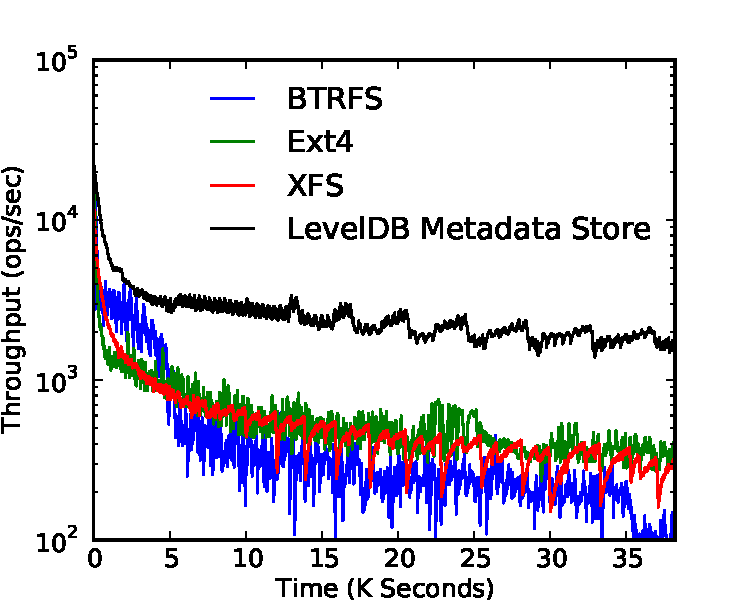
\includegraphics[scale=0.45]{./figs/ldb_insertrate_onenode}}
\caption{
{\small 
Single-node \ldb{}-based metadata store is 10X faster than modern Linux
filesystems for a workload that creates 100 million zero-length files.
X-axis only shows the time until LevelDB finished all insertions because the other 
file systems were much slower. Y-axis is in logarithmic scale.
}
}
\vspace{15pt}
\hrule 
\label{graph:ldb-singlenode}
\end{figure}       %%%%%%%%%%%%%%%%%%%%%%%

\begin{figure}[t]  %%%%%%%%%%%%%%%%%%%%%%%
\centerline{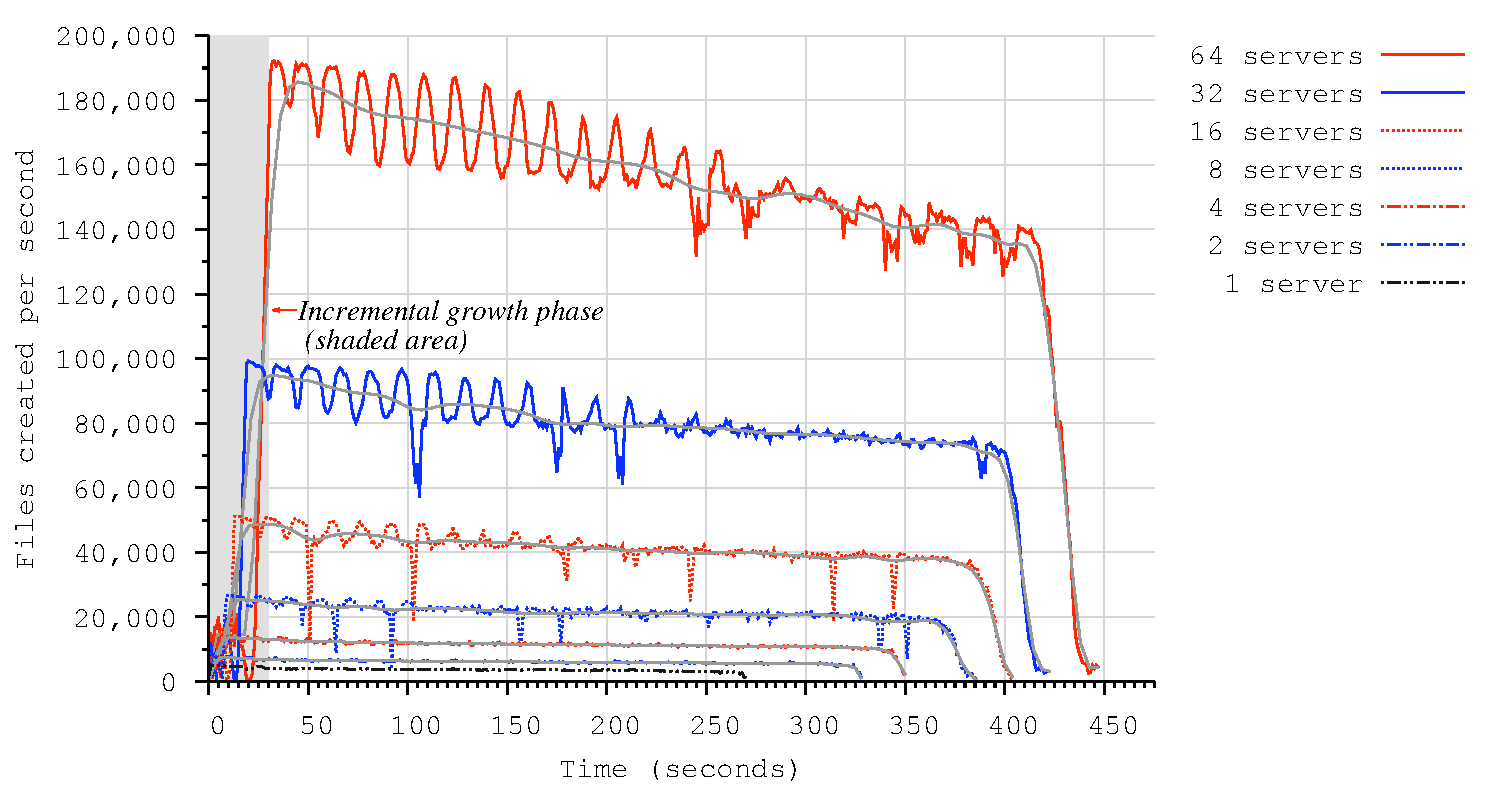
\includegraphics[scale=0.33]{./figs/ldb_insertrate}}
\caption{
{\small
Our middleware metadata service prototype shows promising scalability
up to 64 servers. However the interaction between LevelDB's compaction policies and 
the Linux Ext3's implementation policies causes periodic throughput variance
that degrades as the the number of directory entries in each LevelDB
increases. \textit{Note that the solid lines in each configuration are Bezier
curves to smooth the variability.}
}
}
\vspace{15pt}
\hrule 
\label{graph:ldb-scaling}
\end{figure}       %%%%%%%%%%%%%%%%%%%%%%%

Figure \ref{graph:ldb-scaling} shows the instantaneous throughput during the 
\textit{concurrent create} workload in a strong scaling experiment, i.e.
creating 1 million files per server and reaching up to 64 million files in the
64 server configuration.
The main result in this figure is that as the number of servers doubles the
throughput of the system also scales up. With 64 servers, \giga{} can achieve a
peak throughput of about 190,000 file creates per second. The system delivers
this peak performance after the directory workload has been spread among all
servers.
Before reaching steady-state, the throughput grows gradually due to the splitting
policies adopted by \giga{}.
 
Another observation in Figure \ref{graph:ldb-scaling} is that the system is
unable to sustain the steady-state peak throughput as in the single node test 
shown in in Figure \ref{graph:ldb-singlenode}: 
in fact, in large setups with 8 or more servers, 
the peak throughput drops by as much as 25\% (in case of the 64-server setup).
This is because when there are more entries existing entries, 
it requires more work to make \ldb balance when inserting a new entry.
In theory, the work of inserting a new entry to a LSM tree is $O(\log_{B}(n))$
where $n$ is the total number of inserted entries, and $B$ is a constant factor
proportional to the average number of entries transferred in each disk request. 
Thus we can use the formula $\frac{a\cdot S+b}{\log{T}}$ to
approximate the throughput timelines in Figure \ref{graph:ldb-scaling},
where $S$ is the number of servers, $T$ is the time, and $a$ as well as $b$ 
are constant factors relative to the disk speed and splitting overhead.
By using this estimation, after inserting 64 billion files with 64 servers,
the system still sustains insertion rate at the speed of about 60,000 operations per second.

\begin{comment}
The first reason is periodic \textit{compactions} in LevelDB that create
ordered files 
by periodically sorting the in-memory log and writing them to separate files 
on-disk. If there are pre-existing files from previous compactions, LevelDB merges 
these old files with newly arrived in-memory logs to write out most recent sorted 
sequential files. These compactions cause both read and write disk I/O:
existing sorted files are read into memory and newly merged files are written
back to disks. Figure \ref{graph:ldb-singlenode} shows the variability in insert
throughput of a single node instance of LevelDB-based backend. This figure
shows that periodic background compactions happen during the entire experiment
which causes the throughput to drop steadily -- the overall throughput drop is
more than 35\% of the peak throughput.
In Figure \ref{graph:ldb-scaling}, the throughput drop is much higher in
aggregate but is about the same fraction as the single-node degradation.
This is expected because each LevelDB instance performs these compactions, and 
because each \giga{} server handles a uniform load, all LevelDB instances are busy
performing compactions.  

The second reason for the degrading saw-tooth behavior in Figure
\ref{graph:ldb-scaling} is due to the choice of LevelDB key used by \tfs{}.
Recall that \tfs{} uses a combination of the file name, the parent directory's
unique identifier and the hash value of the file name as the key. 
The hash value of the file name causes an interesting tradeoff: it simplifies
LevelDB's split optimizations but it makes LevelDB's compactions more I/O
intensive.
Because the hash values are uniformly random, even two lexicographically
similar file names in the same parent directory will have random, and
lexicographically very different, hash values.
This makes the entire LevelDB key lexicographically different which causes
LevelDB to read more files during compactions.

To confirm our hypothesis, we compared the variability in LevelDB's insert
throughput for different keys.
Figure "comingInTheFuture" will hopefully how this tradeoff (XXX).
%XXX: function of different keys and values 
\end{comment}

